\documentclass[aspectratio=169]{../latex_main/tntbeamer}  % you can pass all options of the beamer class, e.g., 'handout' or 'aspectratio=43'
\usepackage{dsfont}
\usepackage{bm}
\usepackage[english]{babel}
\usepackage[T1]{fontenc}
%\usepackage[utf8]{inputenc}
\usepackage{graphicx}
\graphicspath{ {./figures/} }
\usepackage{algorithm}
\usepackage[ruled,vlined,algo2e,linesnumbered]{algorithm2e}
\usepackage{hyperref}
\usepackage{booktabs}
\usepackage{mathtools}

\usepackage{amsmath,amssymb}

\DeclareMathOperator*{\argmax}{arg\,max}
\DeclareMathOperator*{\argmin}{arg\,min}

\usepackage{amsbsy}
\newcommand{\vect}[1]{\bm{#1}}
%\newcommand{\vect}[1]{\boldsymbol{#1}}

\usepackage{pgfplots}
\pgfplotsset{compat=1.16}
\usepackage{tikz}
\usetikzlibrary{trees} 
\usetikzlibrary{shapes.geometric}
\usetikzlibrary{positioning,shapes,shadows,arrows,calc,mindmap}
\usetikzlibrary{positioning,fadings,through}
\usetikzlibrary{decorations.pathreplacing}
\usetikzlibrary{intersections}
\pgfdeclarelayer{background}
\pgfdeclarelayer{foreground}
\pgfsetlayers{background,main,foreground}
\tikzstyle{activity}=[rectangle, draw=black, rounded corners, text centered, text width=8em]
\tikzstyle{data}=[rectangle, draw=black, text centered, text width=8em]
\tikzstyle{myarrow}=[->, thick, draw=black]

% Define the layers to draw the diagram
\pgfdeclarelayer{background}
\pgfdeclarelayer{foreground}
\pgfsetlayers{background,main,foreground}

% Requires XeLaTeX or LuaLaTeX
%\usepackage{unicode-math}

\usepackage{fontspec}
%\setsansfont{Arial}
\setsansfont{RotisSansSerifStd}[ 
Path=../latex_main/fonts/,
Extension = .otf,
UprightFont = *-Regular,  % or *-Light
BoldFont = *-ExtraBold,  % or *-Bold
ItalicFont = *-Italic
]
\setmonofont{Cascadia Mono}[
Scale=0.8
]

% scale factor adapted; mathrm font added (Benjamin Spitschan @TNT, 2021-06-01)
%\setmathfont[Scale=1.05]{Libertinus Math}
%\setmathrm[Scale=1.05]{Libertinus Math}

% other available math fonts are (not exhaustive)
% Latin Modern Math
% XITS Math
% Libertinus Math
% Asana Math
% Fira Math
% TeX Gyre Pagella Math
% TeX Gyre Bonum Math
% TeX Gyre Schola Math
% TeX Gyre Termes Math

% Literature References
\newcommand{\lit}[2]{\href{#2}{\footnotesize\color{black!60}[#1]}}

%%% Beamer Customization
%----------------------------------------------------------------------
% (Don't) Show sections in frame header. Options: 'sections', 'sections light', empty
\setbeamertemplate{headline}{empty}

% Add header logo for normal frames
\setheaderimage{
	% 
\includegraphics[height=\logoheight]{figures/TNT_darkv4.pdf}
	
\includegraphics[height=\logoheight]{../latex_main/figures/luh_logo_rgb_0_80_155.pdf}
	% 
\includegraphics[height=\logoheight]{figures/logo_tntluh.pdf}
}

% Header logo for title page
\settitleheaderimage{
	% 
\includegraphics[height=\logoheight]{figures/TNT_darkv4.pdf}
	
\includegraphics[height=\logoheight]{../latex_main/figures/luh_logo_rgb_0_80_155.pdf}
	% 
\includegraphics[height=\logoheight]{figures/logo_tntluh.pdf}
}

% Title page: tntdefault 
\setbeamertemplate{title page}[tntdefault]  % or luhstyle
% Add optional title image here
%\addtitlepageimagedefault{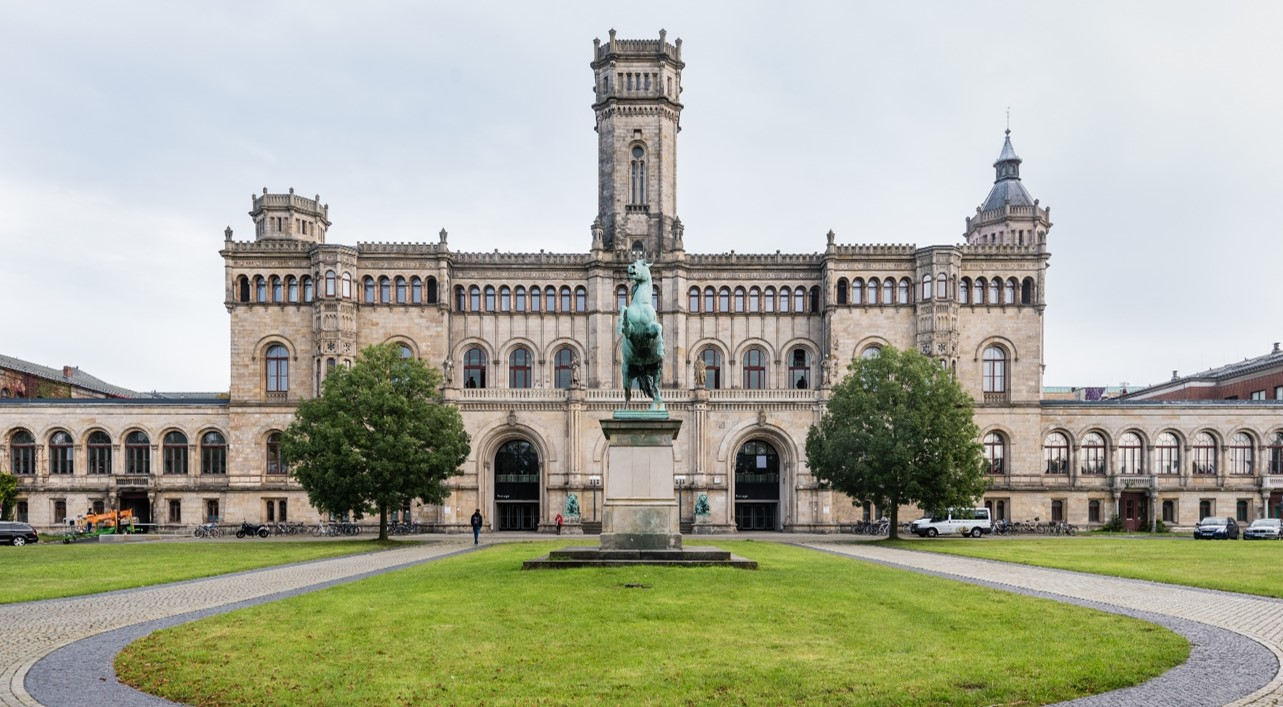
\includegraphics[width=0.65\textwidth]{figures/luh_default_presentation_title_image.jpg}}

% Title page: luhstyle
% \setbeamertemplate{title page}[luhstyle]
% % Add optional title image here
% \addtitlepageimage{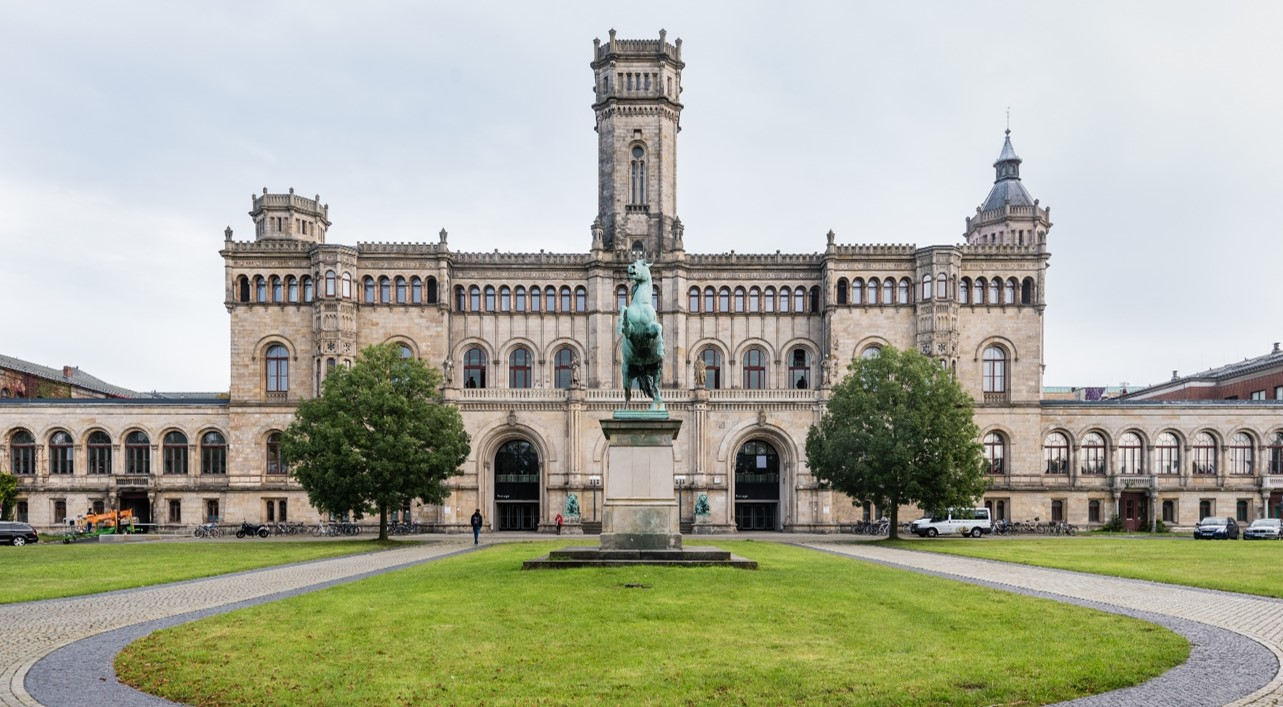
\includegraphics[width=0.75\textwidth]{figures/luh_default_presentation_title_image.jpg}}

\author[Abedjan \& Lindauer]{Ziawasch Abedjan \& Marius Lindauer\\[1em]
	
\includegraphics[height=\logoheight]{../latex_main/figures/luh_logo_rgb_0_80_155.pdf}\qquad
	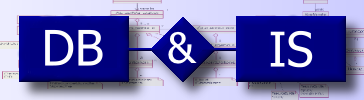
\includegraphics[height=\logoheight]{../latex_main/figures/DBIS_Kurzlogo.png}\qquad

\includegraphics[height=\logoheight]{../latex_main/figures/TNT_darkv4}\qquad

\includegraphics[height=\logoheight]{../latex_main/figures/L3S.jpg}	}
\date{Summer Term 2022; \hspace{0.5em} {
\includegraphics[height=1.5em]{../latex_main/figures/Cc-by-nc-sa_icon.svg.png}}; based on \href{https://ds100.org/fa21/}{[DS100]}
}


%%% Custom Packages
%----------------------------------------------------------------------
% Create dummy content
\usepackage{blindtext}

% Adds a frame with the current page layout. Just call \layout inside of a frame.
\usepackage{layout}


%%% Macros
%\renewcommand{\vec}[1]{\mathbf{#1}}
% \usepackage{bm}
%\let\vecb\bm

\title[Visualization]{DS: Visualization}
\subtitle{Smoothing}

\graphicspath{ {./figure/} }
%\institute{}


\begin{document}
	
	\maketitle
	\begin{frame}{Smoothing}
	    \begin{columns}
	        \begin{column}{.6\textwidth}
	               \begin{itemize}
	                   \item Histograms are a smoothed version of rug plots.
	                   \item We smooth if we want to focus on general structure rather than individual observations.
	               \end{itemize} 
	        \end{column}
	        
	        
	        \begin{column}{.5\textwidth}

	                    \centering
	                    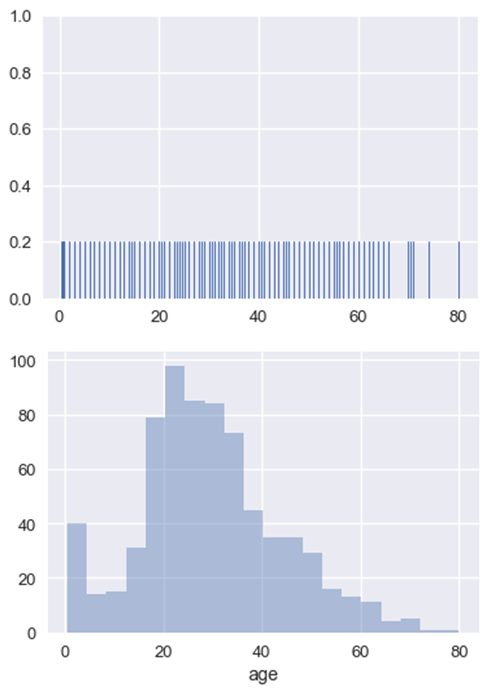
\includegraphics[scale=.32]{Bild82}

	        \end{column}
	    \end{columns}
	\end{frame}
	
	
	\begin{frame}{Spreading proportion uniformly}
	    \begin{columns}
	        \begin{column}{.55\textwidth}
	        
	            Points:  [2.2, 2.8, 3.7, 5.3, 5.7]\\
                Bins: [0, 2), [2, 4), [4, 6), [6, 8]

	               \begin{itemize}
	                   \item Each of the 5 points is a proportion $\frac{1}{5}$ of the list.
	                   \item In a histogram, area = proportion.
	                   \item Each point:
	                   \begin{itemize}
	                       \item Contributes an area 1/5 to the histogram.
	                       \item Rectangle has width 2 and thus height 1/10. 
	                   \end{itemize}
	                   \item Kernel density estimates follow similar guidelines.
	               \end{itemize} 
	        \end{column}
	        
	        
	        \begin{column}{.5\textwidth}

	                    \centering
	                    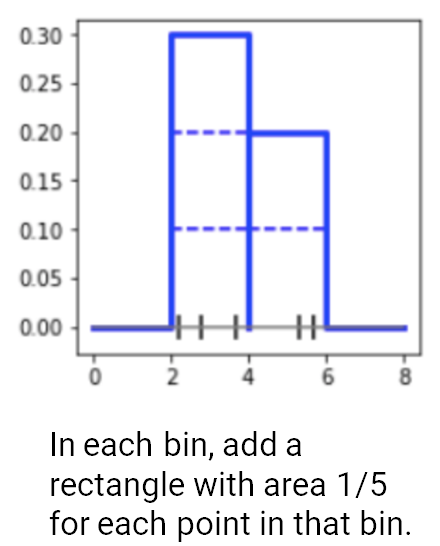
\includegraphics[scale=.4]{Bild83}

	        \end{column}
	    \end{columns}
	\end{frame}
	
	
	\begin{frame}{Kernel density estimation (KDE)}
	    \begin{columns}
	        \begin{column}{.5\textwidth}
	            	    Kernel Density Estimation is used to estimate a probability density function (or density curve) from a set of data.

	               \begin{itemize}
	                   \item Just like a histogram, a density function’s total area must sum to 1.
	               \end{itemize}
	               To create a KDE:
	               \begin{itemize}
	                   \item Place a kernel at each data point.
	                   \item Normalize kernels so that total area = 1.
	                   \item Sum all kernels together.
	               \end{itemize}
	               We also need to choose a kernel and bandwidth.
	        \end{column}
	        
	        
	        \begin{column}{.5\textwidth}
	                \begin{figure}
	                    \centering
	                    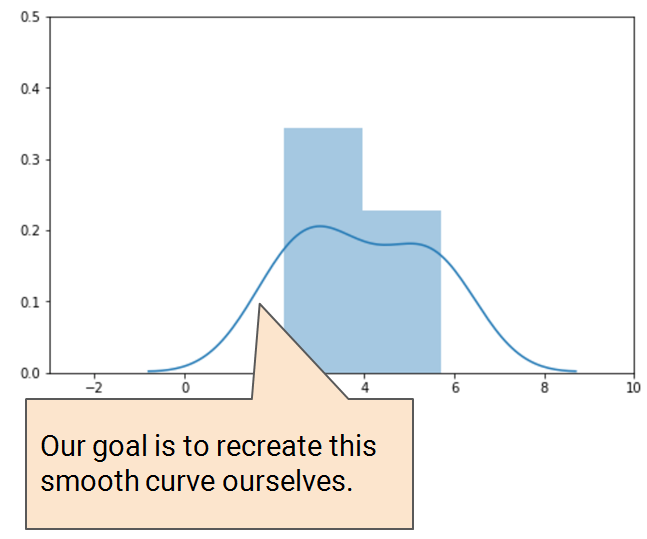
\includegraphics[scale=.4]{Bild84}
	                \end{figure}
	        \end{column}
	    \end{columns}
	\end{frame}
	
	
	\begin{frame}{Step 1 – place a kernel at each data point}
	    At each of our 5 points (depicted in the rug plot on the left), we’ve placed a Gaussian kernel with alpha = 1. The idea is that there is a higher density near the points we’ve already seen.
	    \begin{figure}
	        \centering
	        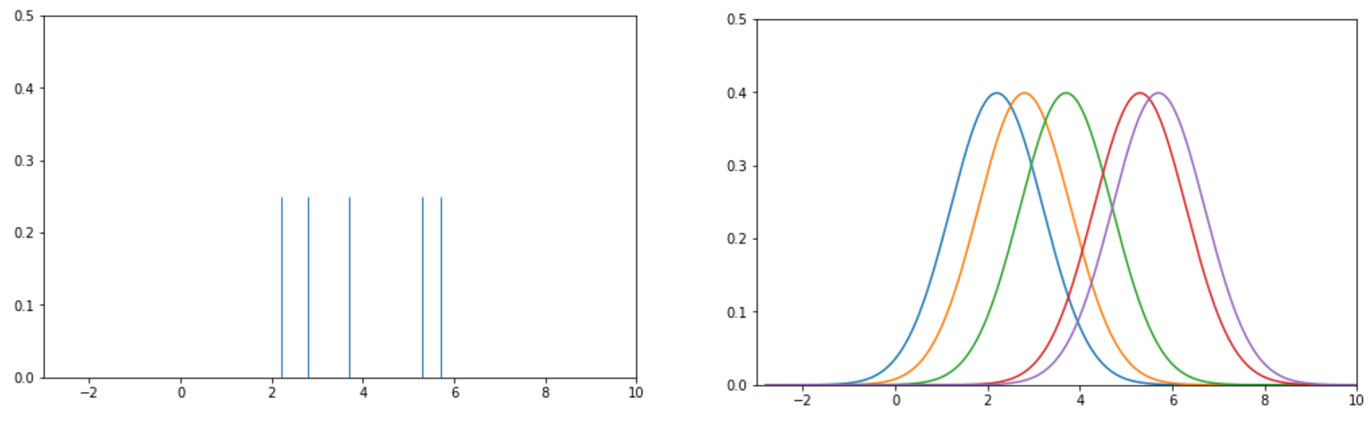
\includegraphics[scale=.4]{Bild85}
	    \end{figure}
	\end{frame}
	
	
	\begin{frame}{Step 2 – normalize kernels}
	    In Step 3, we will be summing each of these kernels. We want the result to be a valid density, that has area 1. Right now, we have 5 different kernels, each with an area 1. So, we multiply each by 1/5.
	    \begin{figure}
	        \centering
	        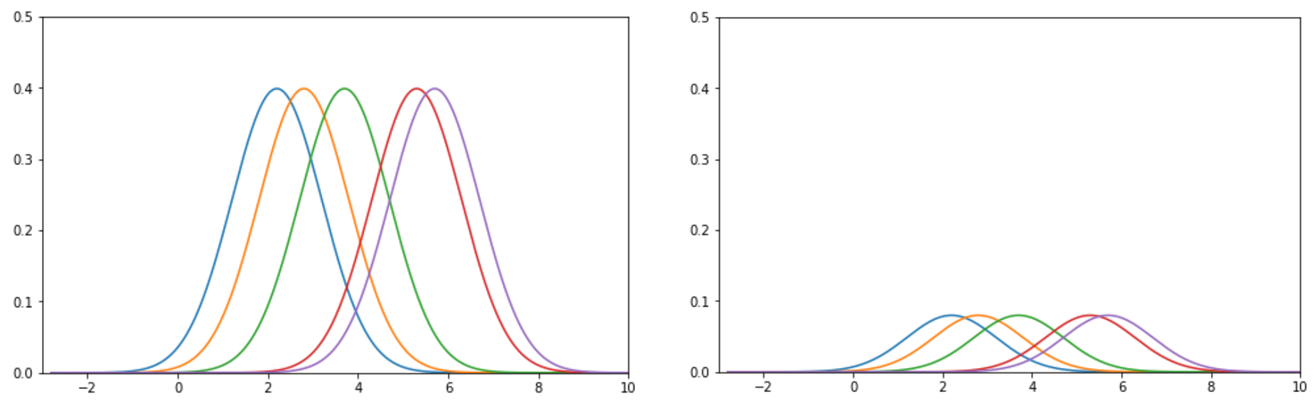
\includegraphics[scale=.4]{Bild86}
	    \end{figure}
	\end{frame}
	
	
	\begin{frame}{Step 3 – sum kernels}
	    Our kernel density estimate is the sum of the normalized kernels at each point. It is depicted below on the right.
	    \begin{figure}
	        \centering
	        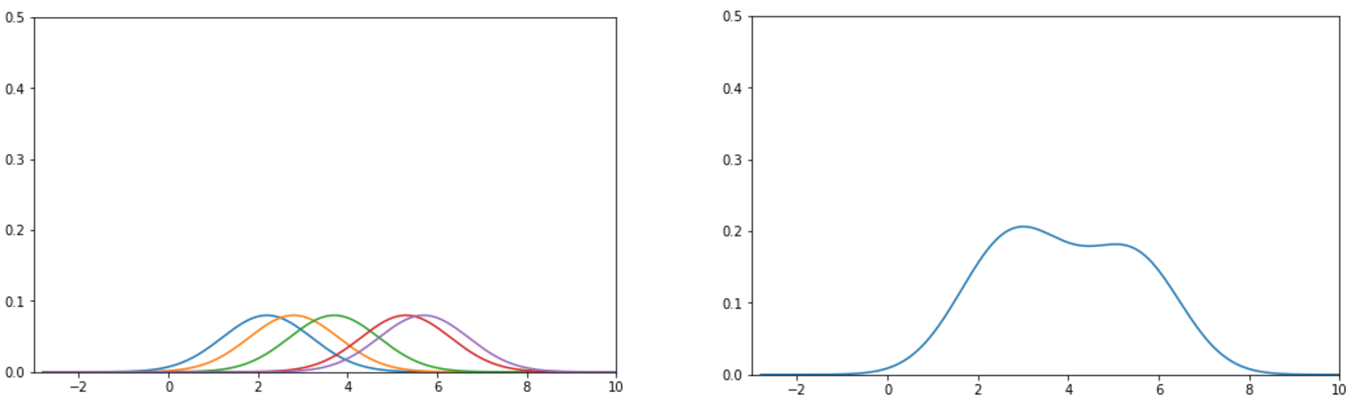
\includegraphics[scale=.4]{Bild87}
	    \end{figure}
	\end{frame}
	
	
	
	\begin{frame}{Kernel density estimates (KDE)}
	    The curve we manually created (left) exactly matches the one that \texttt{sns.distplot} creates for us (right)!
	    \begin{figure}
	        \centering
	        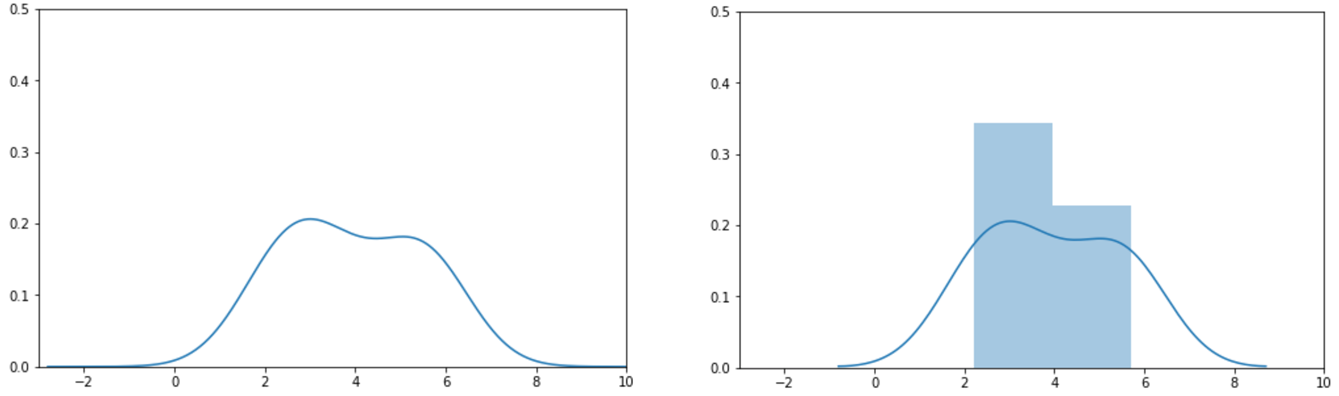
\includegraphics[scale=.4]{Bild88}
	    \end{figure}
	\end{frame}
	
	
	\begin{frame}{Kernels}
	    \begin{itemize}
	        \item A kernel (for our purposes) is a valid density function. That means it:
	        \begin{itemize}
	            \item Must be non-negative for all inputs.
	            \item Must integrate to 1.
	        \end{itemize}
	        \item The most common kernel is the Gaussian kernel.
	        \begin{itemize}
	            \item Here, $x$ represents any input, and $x_i$ represents the ith observed value. The kernels are centered on our observed values (and so the mean of this distribution is $x_i$).
	            \item $\alpha$ is the bandwidth parameter. It controls the smoothness of our KDE. Here, it is also the standard deviation of the Gaussian.
	        \end{itemize}
	    \end{itemize}
	    
	    \begin{equation*}
	        K_\alpha (x,x_i) = \frac{1}{\sqrt{2\pi\alpha^2}}e^{-\frac{(x-x_i)^2}{2\alpha^2}}
	    \end{equation*}
	\end{frame}
	
	
	
% 	\begin{frame}{Boxcar Kernel}
	
% 	    \begin{columns}
	    
% 	        \begin{column}{.5\textwidth}
	        
% 	                \begin{itemize}
% 	                    \item Another common kernel is the boxcar kernel.
% 	                    \begin{itemize}
% 	                        \item It assigns uniform density to points within a “window” of the observation, and 0 elsewhere.
% 	                        \item Resembles a histogram… sort of.
% 	                    \end{itemize}
% 	                \end{itemize}
% 	                \begin{equation*}
% 	                    K_\alpha (x,x_i) = \left\{\begin{array}{cc}
% 	                        \frac{1}{\alpha}, & |x-x_i| \leq \frac{\alpha}{2} \\
% 	                        0, & \text{else}
% 	                    \end{array}\right.
% 	                \end{equation*}

% 	                    \centering
% 	                    \vspace{-3em}
% 	                    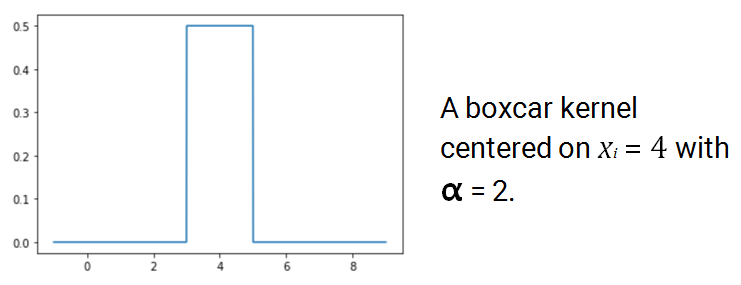
\includegraphics[scale=.35]{Bild90}
	                
% 	        \end{column}
	        
	        
% 	        \begin{column}{.5\textwidth}
	        
% 	                    \centering
% 	                    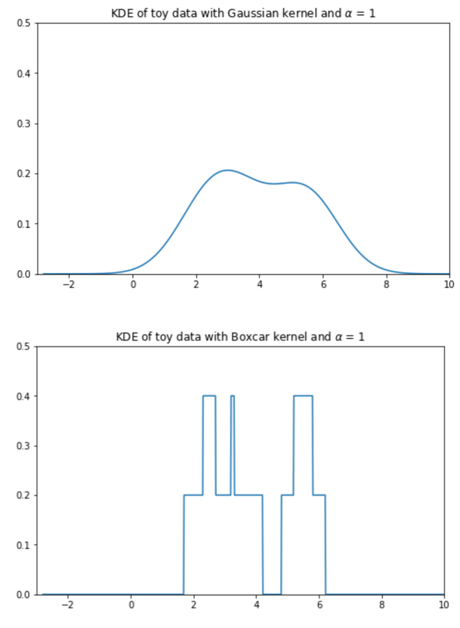
\includegraphics[scale=.35]{Bild89}

% 	        \end{column}
	        
% 	    \end{columns}
	    
	    
% 	\end{frame}
	
	
	\begin{frame}{Effect of bandwidth on KDEs}
	    \begin{columns}
	        \begin{column}{.5\textwidth}

	                    \centering
	                    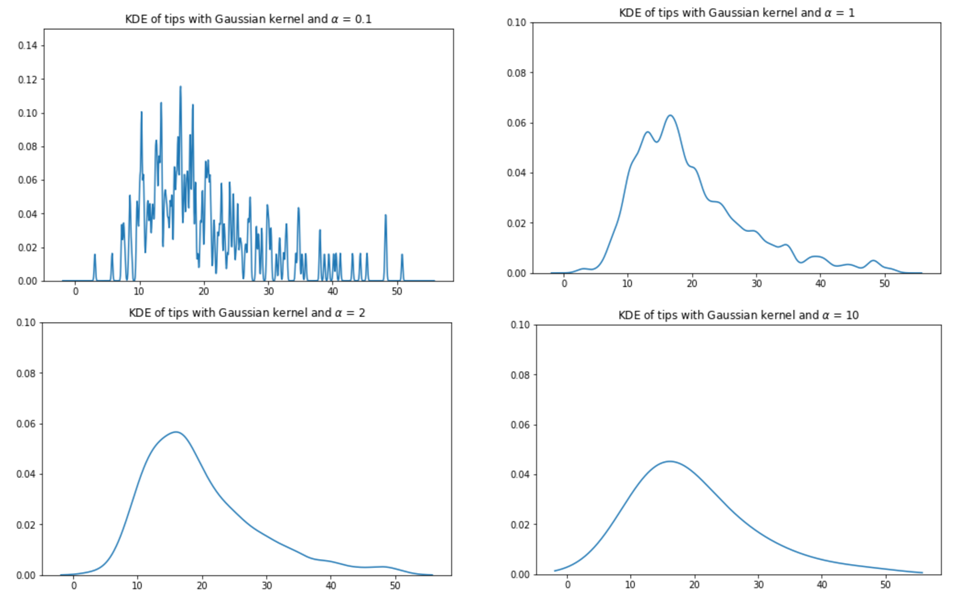
\includegraphics[scale=.3]{Bild91}

	        \end{column}
	        
	        
	        \begin{column}{.5\textwidth}

                    \vspace{-2em}
	                Bandwidth is analogous to the width of each bin in a histogram.
	                \begin{itemize}
	                    \item As $\alpha$ increases, the KDE becomes more smooth.
	                    \item Simpler to understand, but gets rid of potentially important distributional information.
	                    \item We call $\alpha$ a \alert{hyperparameter}. Be familiar with this term!
	                \end{itemize}
	                    \centering
	                    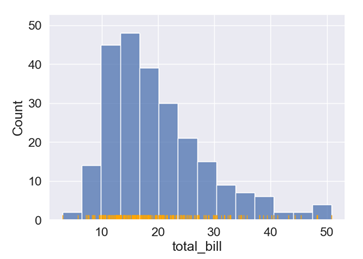
\includegraphics[scale=.28]{Bild92}

	        \end{column}
	    \end{columns}
	\end{frame}
	
	
	\begin{frame}{Summary of KDE}
	    \begin{equation*}
	        f_\alpha (x) = \frac{1}{n}\sum_{i=1}^n K_\alpha (x,x_i)
	    \end{equation*}
	    The “KDE formula” is above.
	    \begin{itemize}
	        \item $x$ represents any number on the number line. It is the input to our function.
	        \item n is the number of observed data points that we have.
	        \item Each $x_i$ ($x_1$, $x_2$, …, $x_n$) represents an observed data point.\\ These are what we use to create our KDE.
	        \item $\alpha$ is the bandwidth or smoothing parameter.
	        \item $K_\alpha(x, x_i)$ is the kernel centered on the i-th observation. 
            \begin{itemize}
                \item Each kernel individually has area 1. We multiply by 1/n so that the total area is still 1.
            \end{itemize}
	    \end{itemize}
	\end{frame}
	
	
	
	\begin{frame}{Extensions}
	
	  \begin{columns}
	   \begin{column}{.5\textwidth}
	   
	    \begin{itemize}
	        \item One can extend the idea of kernel density estimation to two dimensions.
	        \begin{itemize}
	            \item A contour plot is a two dimensional KDE (top).
	        \end{itemize}
	        
	        \vspace{3em}
	        \item One can also use kernels to create smoothed versions of scatterplots (bottom).

	    \end{itemize}
	    
	    \end{column} 
	    
	    \begin{column}{.5\textwidth}
	    
	               \centering
	               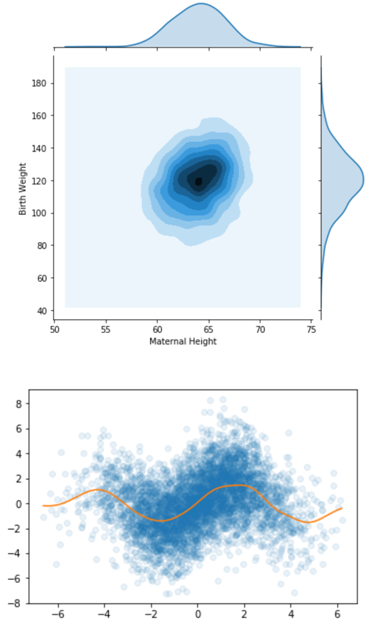
\includegraphics[scale=.35]{Bild93}

	    \end{column}
	    
	   \end{columns}
	\end{frame}
\end{document}